% !TeX spellcheck = en_US
\addsection{Random Scenario}{\images/random.png}

\begin{multicols*}{2}

\textit{As dice roll and fortunes shift, the lands of Antagarich spread before you in all their splendor.
  Your destiny follows these celestial rolls, each battle and treasure determined by chance.
  Will you emerge victorious in this battle royale, claim the sacred grail, or stand alone as the king of the hill when the final die settles?
}

Instead of playing a specific Scenario, you can follow these guidelines to create a random one.
Of course, you can adjust everything at will.

\subsection*{\MakeUppercase{Scenario Type}}

Choose one of the following types for your play:

\textbf{Battle Royale} -- Win by eliminating your opponents or gaining more Victory Points (VPs) than them.
VPs are counted in accordance to the Tournament book.
Additionally, you get:
\begin{itemize}
  \item 5 VPs for flagging a Dragon Utopia for the first time.
  \item 2 VPs for controlling the Dragon Utopia at the end of the game.
  \item 5 VPs for bringing the Grail to your faction Town \textit{OR} 3 VPs for owning the Grail  at the end of the game.
\end{itemize}

\textbf{King of the Hill} -- Start a map with a Dragon Utopia in the middle.
You don't need to fight the Level 7 Combat to capture it.
1 VP for each Round you hold the Dragon Utopia under your control, no VPs from anything else.

\textbf{Capture the Grail} -- Start a map with the Grail in the middle.
Standard Grail rules apply: spend 2 \svgeven{movement} to dig it up, and bring it to your Town.
\vspace*{\fill}
\columnbreak

\subsection*{\MakeUppercase{Scenario Length\\and Map Size}}

Depending on your apetite, each player gets:

\textbf{Small Map:} 8 Rounds
\begin{itemize}
  \item 1 × Starting (I) Map Tile
  \item 2 × Far (II-III) Map Tile
\end{itemize}

\textbf{Medium Map:} 12 Rounds
\begin{itemize}
  \item 1 × Starting (I) Map Tile
  \item 2 × Far (II-III) Map Tile
  \item 1 × Near (IV-V) Map Tile
\end{itemize}

\textbf{Large Map:} 16 Rounds
\begin{itemize}
  \item 1 × Starting (I) Map Tile
  \item 2 × Far (II-III) Map Tile
  \item 2 × Near (IV-V) Map Tile
\end{itemize}

\subsection*{\MakeUppercase{Map Setup}}

Decide player order before placing the Tiles.
In reverse player order, each player places one Tile in descending level (Near \rightarrow\ Far \rightarrow\ Starting).

\begin{tikzpicture}[overlay]
  \node[inner sep=0pt, opacity=0.2, xscale=-1, rotate=12] at (3, -4.4) {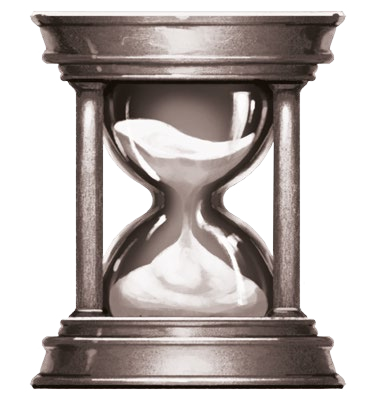
\includegraphics[width=0.85\linewidth, keepaspectratio]{\art/hourglass.png}};
\end{tikzpicture}

\end{multicols*}

\subsection*{\MakeUppercase{Player Setup}}

Choose your \textbf{starting conditions} and \textbf{Town strength}.

\let\origbronze\bronze
\let\origsilver\silver
\let\origgolden\golden
\let\origazure\azure
\renewcommand{\bronze}{\origbronze[12]}
\renewcommand{\silver}{\origsilver[12]}
\renewcommand{\golden}{\origgolden[12]}
\renewcommand{\azure}{\origazure[12]}


\hommtable[]{27}{
  \centering
  \medskip
  \textbf{Starting Conditions}\\
  \bigskip

  \begin{tabularx}{0.99\linewidth}{p{0.12\linewidth}XXXX} & \darkcell{Stingy} & \darkcell{Fair} & \darkcell{Generous}\\
  \darkcell[1.4]{Army}
    & \lightcellleft[1.4]{2 × Few cheaptes \bronze\ Units}
    & \lightcellleft[1.4]{Pack of cheap \bronze\ Units \linebreak Few pricy \bronze\ Units}
    & \lightcellleft[1.4]{Pack of pricy \bronze\ Units \linebreak Few cheap \silver\ Units}\\
  \darkcell[1.4]{Starting Resources}
    & \lightcellleft[1.4]{10 \svg{gold}, 3 \svg{building_materials}, 1 \svg{valuables}}
    & \lightcellleft[1.4]{16 \svg{gold}, 5 \svg{building_materials}, 1 \svg{valuables}}
    & \lightcellleft[1.4]{20 \svg{gold}, 8 \svg{building_materials}, 2 \svg{valuables}}\\
  \end{tabularx}

  \bigskip
  {\color{yellow}\rule{\linewidth}{1pt}}

  \vspace*{1em}
  \textbf{Town Strength}\\
  \bigskip

  \begin{tabularx}{0.99\linewidth}{p{0.12\linewidth}XXXX} & \darkcell{Settlement} & \darkcell{City} & \darkcell{Capitol}\\
  \darkcell[1.4]{Starting Income}
    & \lightcellleft[1.4]{10 \svg{gold}, 0 \svg{building_materials}, 0 \svg{valuables}}
    & \lightcellleft[1.4]{15 \svg{gold}, 0 \svg{building_materials}, 1 \svg{valuables}}
    & \lightcellleft[1.4]{20 \svg{gold}, 2 \svg{building_materials}, 1 \svg{valuables}}\\
  \darkcell[2.0]{Town Buildings}
    & \lightcellleft[2.0]{\bronze\ Dwelling}
    & \lightcellleft[2.0]{\bronze\ Dwelling \linebreak City Hall}
    & \lightcellleft[2.0]{\bronze\ Dwelling \linebreak City Hall \linebreak Citadel}\\
  \end{tabularx}
}
